\section{Iterative Learning Control with Movement Primitives}\label{method}

In a highly dynamic and complex task such as robot table tennis, one often needs to consider an extension of the standard trajectory tracking task. Based on the varying initial positions and velocities of the robot arm and the trajectory of the incoming ball, in each table tennis stroke the robot arm needs to track different trajectories that start from different initial conditions and end with different goal states of the arm. Moreover these trajectories need to be scaled in time to intercept the ball. Dynamic Movement Primitives (DMP) are especially useful for representing such a variety of movement patterns.
% reference needed? revise.

%Sometimes for safety reasons, for instance when interacting with external objects or under unforeseen perturbations \cite{Schaal07}, a \emph{low-gain} feedback law operating on the inputs may be fine-tuned to be compliant. As another practical restriction, one may not even be allowed to modify the low-level controller of the industrial robot \cite{Longman2000}. In such cases, it is not possible to modify the input signals $\sysInput$ directly. Instead one can modify the reference trajectories that are provided to the low-level controllers. It can be shown that this is an equivalent approach to modifying the feedforward control inputs \cite{Bristow06}.

Based on these considerations, in this paper we focus on learning to track DMPs $\vec{\dmp}(t) = [\joint_{\text{des}}(t),\dot{\joint}_{\text{des}}(t)]^{\mathrm{T}}$. An initial DMP might be constructed out of a given demonstration or an optimal reference trajectory $\traj(t)$ using regression techniques \cite{Ijspeert13}. Representing a reference trajectory with movement primitives has some benefits: nonsmooth parts of the trajectory can be filtered, the evolution of desired states can be coupled with errors to ensure safety, time and scaling invariance of the differential equations can be used to adapt the trajectory to task changes in time as well as in space. %Robustness to initial joint position and velocity changes 

\subsection{Movement Primitive Formulation}

Striking movement primitives suited to table tennis have been proposed in \cite{Kober10} and \cite{Muelling13} as an extension of discrete DMPs. Unlike the original formulation~\cite{Ijspeert02}, these extensions allow for an arbitrary velocity profile to be attached to the primitives around hitting time. However, these \emph{ad hoc} approaches are unnecessarily cluttered and involve additional tuning parameters. Arguably they are also against the philosophy behind the discrete primitive: the motion converges necessarily to a goal state with zero velocity. We propose here instead to use rhythmic DMPs that allow for a limit cycle attractor, which is inevitable if we want to maintain the striking motion through goal state. After the striking is completed the DMP can be used to return back to initial state or it can be terminated by setting the forcing terms to zero. An example is shown in Figure~\ref{rdmp}.

The rhythmic movement primitive equations~\cite{Kober08} can each be written as
%
\begin{equation}
\begin{aligned}
\begin{bmatrix}
   \dot{\dmp}_1 \\
   \dot{\dmp}_2
 \end{bmatrix} = \begin{bmatrix}
     \dmp_2  \\
     \alpha_{g} (\beta_{g}\tau^2(\goal - \dmp_1) - \tau\dmp_2) +  \tau^2\force(\phase)
  \end{bmatrix}
\label{dmp},
\end{aligned}
\end{equation}
%
\noindent where the phase $\phase$ evolves as $\dot{\phase} = \tau$. The constant $\tau$ determines the period of the limit cycle and the forcing term $\force$ enforces the limit cycle with $M$ weighted Von-Mises basis functions $\basis_i$
%
\begin{equation}
\begin{aligned}
\force(\phase,\amp) &= \frac{\sum_{i=1}^{M}\basis_i \weights_i}{\sum_{i=1}^{M}\basis_i}\amp, \\
\basis_i &= \exp(\basisHeight_i (\cos(\phase - \basisCenter_i) - 1)).
\label{forcing}
\end{aligned}
\end{equation}
%
\noindent Here $\amp, \basisHeight_i, \basisCenter_i$ determine the amplitude of the motion, the width and the centers of the basis functions respectively.

The dynamical system \eqref{dmp} describes the motion of each of the desired joint states along a particular periodic path in joint space. The forcing terms determine this path by warping the motion of the spring dynamics. The weights $\weights$ are obtained with regression using demonstration data. The spring constants $\alpha_{g}$ and $\beta_{g}$ ensure that starting from any initial position and velocity $\dmp_0$ the DMP converges to the limit cycle with center $\goal$ and are usually chosen such that the dynamical system is critically damped.

Unlike the discrete DMP, the rhythmic DMP is a linear time-varying system and adaptions of target positions and velocities can be easily performed. Using linear systems theory one can show the feasibility of such adaptations and construct phase-dependent modifications of the DMP parameters $\goal,\amp$.

% a figure showing convergence from different starting conditions needed here
\begin{figure}
\center
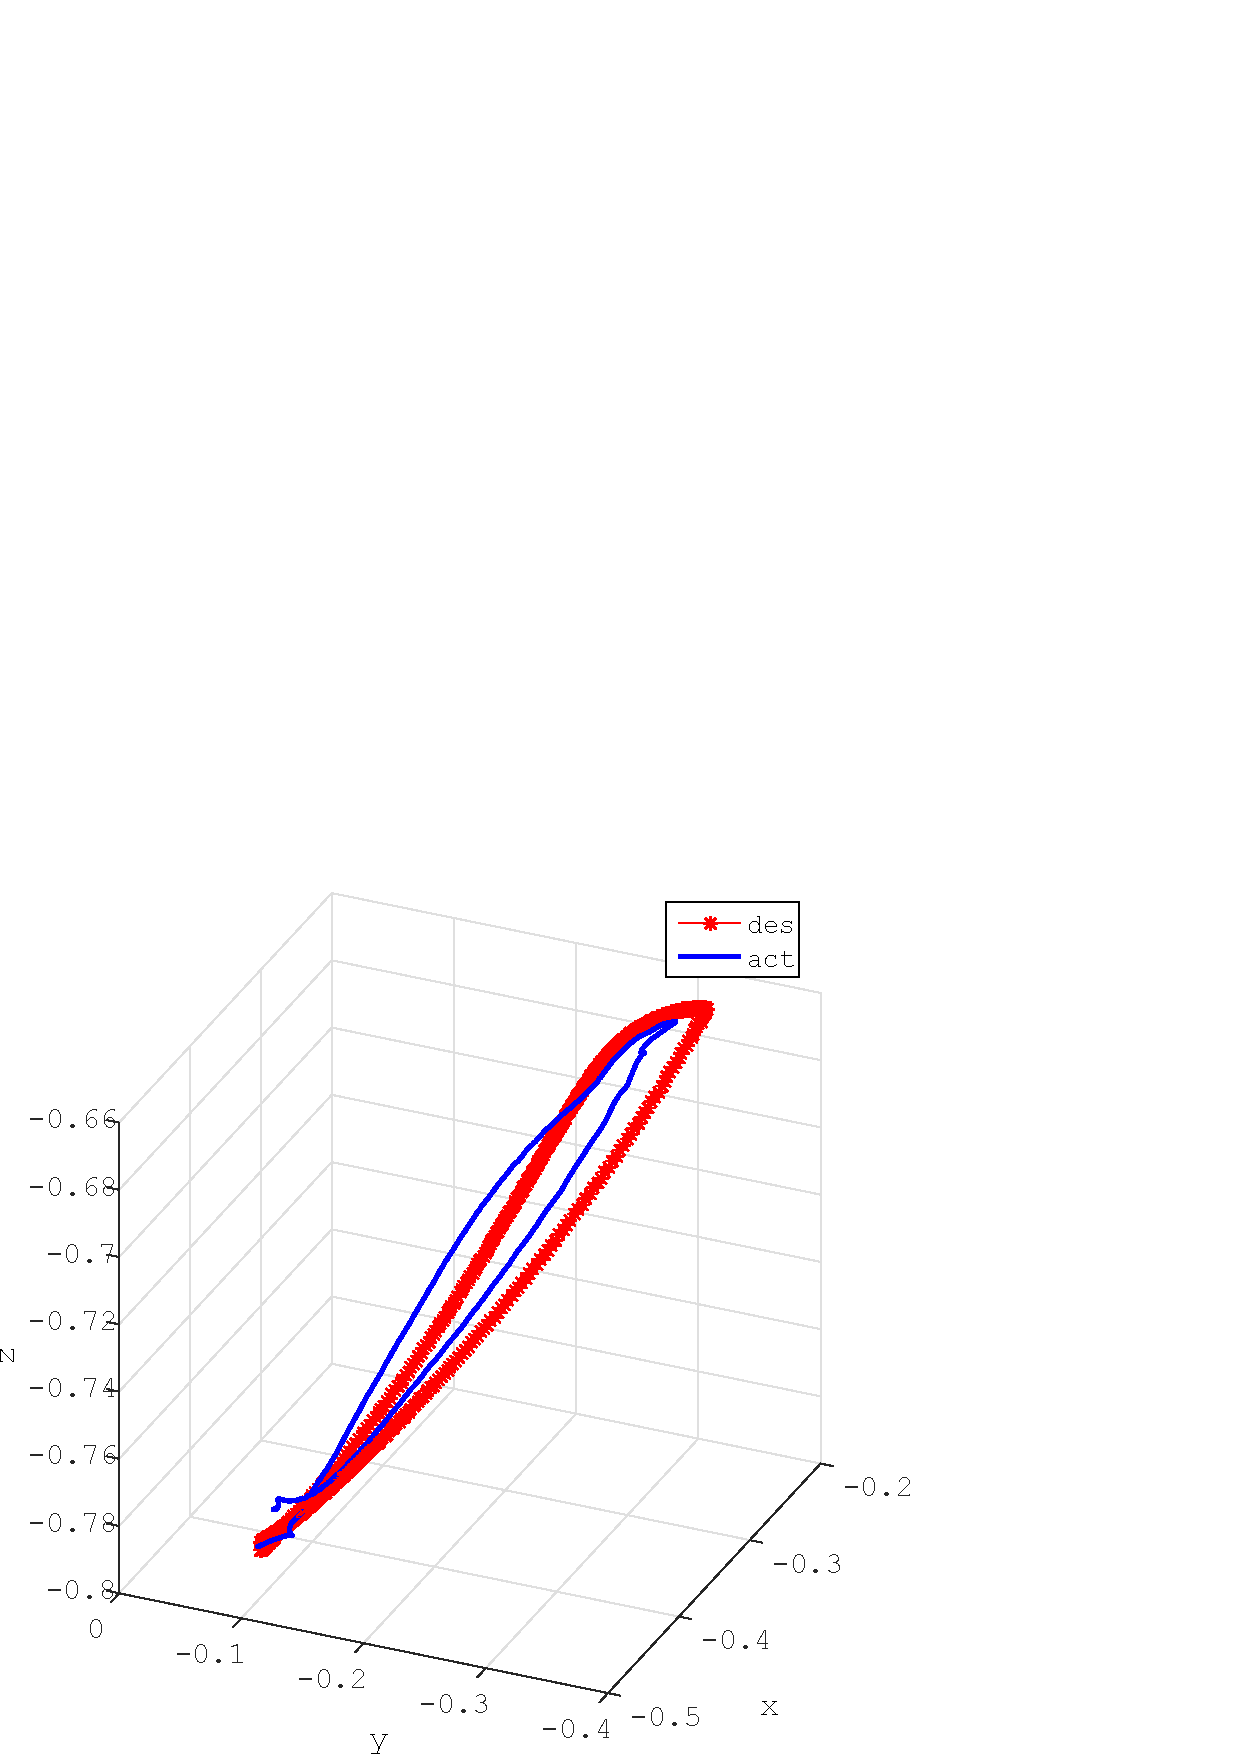
\includegraphics[scale=0.30]{rdmp.pdf}
%\scalebox{1.0}{% This file was created by matlab2tikz v0.4.4 running on MATLAB 8.0.
% Copyright (c) 2008--2013, Nico Schlmer <nico.schloemer@gmail.com>
% All rights reserved.
% 
% The latest updates can be retrieved from
%   http://www.mathworks.com/matlabcentral/fileexchange/22022-matlab2tikz
% where you can also make suggestions and rate matlab2tikz.
% 
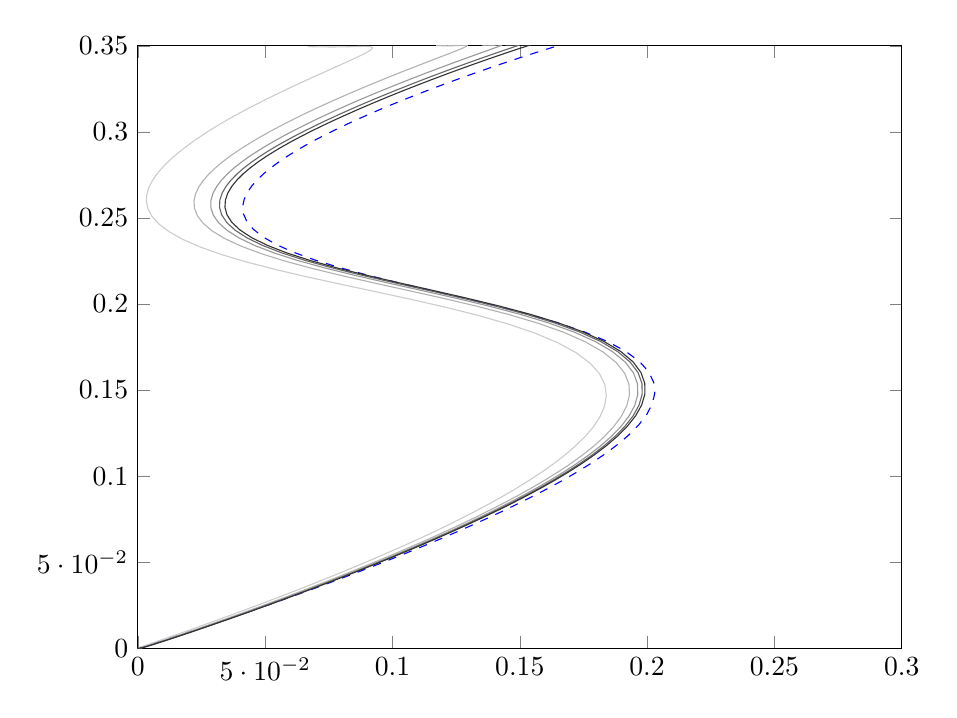
\begin{tikzpicture}

\begin{axis}[%
width=0.8\columnwidth,
height=0.630967741935484\columnwidth,
scale only axis,
xmin=0,
xmax=0.3,
ymin=0,
ymax=0.35
]
\addplot [
color=blue,
dashed,
forget plot
]
table[row sep=crcr]{
-1.22568529189217e-17 1.70219232680293e-47\\
-1.22078040529282e-17 2.17466204815869e-20\\
1.24930069097586e-15 5.59329658828069e-16\\
4.31962537102899e-13 1.9152423618868e-13\\
2.51770978879146e-11 1.11631432791867e-11\\
5.55015544523879e-10 2.46106431437956e-10\\
6.60280135771012e-09 2.9283319802688e-09\\
5.12320770129383e-08 2.27281407753508e-08\\
2.90255123674167e-07 1.28827401032052e-07\\
1.29124388293531e-06 5.73511237251698e-07\\
4.73949589296885e-06 2.10713748978966e-06\\
1.48681255318932e-05 6.6189380207418e-06\\
4.09129882041033e-05 1.82444393148059e-05\\
0.000100718153544017 4.50090857862532e-05\\
0.000225245856791989 0.000100919801590805\\
0.000463240655356511 0.000208196459707293\\
0.000884823147305501 0.000399120180670242\\
0.00158255610123486 0.000716854697447387\\
0.00266870907570527 0.00121464755420377\\
0.0042680934828865 0.00195306659807664\\
0.00650682428145541 0.00299533100932766\\
0.00949841893898853 0.00440125030957139\\
0.0133294488642299 0.00622065804358311\\
0.0180472586508033 0.00848740810159894\\
0.0236519674180277 0.0112149390444555\\
0.0300941529569334 0.0143941271208937\\
0.0372785249971626 0.0179937242124732\\
0.0450728081170337 0.0219632243456565\\
0.0533202318837492 0.0262376267222215\\
0.0618536166580361 0.0307433345872289\\
0.0705090712117028 0.0354043703208843\\
0.0791376965311413 0.0401481768418987\\
0.0876142690996799 0.0449104641836341\\
0.0958424961170963 0.0496387890730672\\
0.10375696557487 0.0542947727843779\\
0.111322280599518 0.0588550337458356\\
0.118530050316482 0.06331102120878\\
0.125394431996405 0.0676679861084513\\
0.131946828905364 0.0719433270169786\\
0.138230198729659 0.0761645191587581\\
0.144293265660084 0.0803667887860157\\
0.150184789161511 0.084590646654827\\
0.155947944238694 0.0888793518508938\\
0.161614820549927 0.0932763463165637\\
0.167201052648133 0.0978226842719481\\
0.172700648861156 0.102554481146252\\
0.178081188148765 0.107500424919056\\
0.183279696817351 0.112679429291778\\
0.188199689821794 0.11809856122523\\
0.192710046988842 0.123751440482291\\
0.196646565585241 0.12961737738435\\
0.199817148084927 0.135661573700226\\
0.202011400876493 0.141836677658674\\
0.20301387722613 0.148085506344443\\
0.202619789967853 0.154344644220661\\
0.20065273345486 0.160548886433011\\
0.196983021746862 0.166636203811203\\
0.191544736744952 0.172552738672092\\
0.184349409899893 0.178257268594913\\
0.175494381526898 0.183724581129977\\
0.165164317442443 0.188947295992029\\
0.153625080784607 0.193935846625374\\
0.1412100661361 0.198716567169214\\
0.12830006671719 0.203328087323888\\
0.115298606077758 0.207816473182085\\
0.10260527646616 0.212229725482657\\
0.0905898807700316 0.216612327368361\\
0.079570030652499 0.221000508160764\\
0.0697943393352088 0.225418764413873\\
0.0614325578259062 0.229877979341309\\
0.0545730774278078 0.234375244026284\\
0.0492273137352959 0.238895250492305\\
0.0453397371877769 0.243412935431724\\
0.0428018209176867 0.247896930561529\\
0.0414679809317703 0.252313332254143\\
0.0411716730700138 0.25662933480681\\
0.0417402386729666 0.260816396765839\\
0.0430079265640447 0.264852853167071\\
0.0448258671359753 0.268725657669276\\
0.0470681659059565 0.272431034965027\\
0.0496347242551211 0.275974250701863\\
0.0524515935766653 0.279368747748684\\
0.0554695907154709 0.282634858417776\\
0.0586617700544091 0.285798252905515\\
0.0620201947143181 0.288888235420426\\
0.0655523003124128 0.291935958228636\\
0.0692770158504934 0.294972594140621\\
0.0732207080290693 0.298027491449363\\
0.0774129544020573 0.301126332090716\\
0.0818821323091202 0.304289323201106\\
0.086650838109129 0.307529473239184\\
0.0917312255322955 0.310851034404806\\
0.0971204675308709 0.314248229434997\\
0.102796687767279 0.317704416545961\\
0.108715848493778 0.321191871765943\\
0.114810181592199 0.324672370955634\\
0.120988762173356 0.328098721508834\\
0.127140705706413 0.3314173160038\\
0.133141194808927 0.33457165455712\\
0.138860120113893 0.33750661939838\\
0.14417260737948 0.340173109510588\\
0.148970203575231 0.342532494031226\\
0.15317114157554 0.344560265930261\\
0.156728025765686 0.346248311683806\\
0.159631560364095 0.347605376663323\\
0.16190957122079 0.348655584952959\\
0.163621436389131 0.349435214610502\\
0.164848937801264 0.349988255460754\\
0.165685237911466 0.350361500346063\\
0.166223974647865 0.350599977591089\\
0.166550272189824 0.350743403168433\\
0.166734851771187 0.350824053127807\\
0.166831595215191 0.350866113799758\\
0.166878121826248 0.350886259282569\\
0.166898406741448 0.350895013534916\\
0.166906302339804 0.350898412202254\\
0.16690899217171 0.35089956776726\\
0.166909773384699 0.350899902896113\\
0.166909959992641 0.350899982867216\\
0.166909994843181 0.350899997792469\\
0.166909999566499 0.350899999814467\\
0.166909999980335 0.350899999991584\\
0.166909999999663 0.350899999999856\\
0.166909999999999 0.3509\\
0.16691 0.3509\\
0.16691 0.3509\\
};
\addplot [
color=white!80!black,
solid,
forget plot
]
table[row sep=crcr]{
-1.22568529189217e-17 1.70219232680293e-47\\
3.25274463507264e-06 8.35905362814104e-08\\
1.23717401990733e-05 6.51809556987925e-07\\
2.60782198962572e-05 2.10499070948953e-06\\
4.3092311772854e-05 4.74258914527822e-06\\
6.21318876894655e-05 8.7637958130708e-06\\
8.19125001256813e-05 1.42692959778432e-05\\
0.000101156688969535 2.12681872858731e-05\\
0.000118643983994053 2.97049649157848e-05\\
0.000133386193364771 3.95467615229986e-05\\
0.00014510004883005 5.10128278393354e-05\\
0.0001552465101183 6.5075416432896e-05\\
0.000168952051477796 8.43854757627399e-05\\
0.000198041564834851 0.000114740042164133\\
0.00026513772561189 0.000167083224948609\\
0.000408333337430968 0.000259824989119074\\
0.000685436662127054 0.000421023858453292\\
0.00117641921404975 0.000689800526123193\\
0.0019826628090404 0.0011163219128708\\
0.00322202345439749 0.00175987161326193\\
0.00501956323556232 0.00268488373870233\\
0.00749484404363355 0.0039552731473001\\
0.0107476267088559 0.00562781764097272\\
0.0148443828740994 0.00774561614639042\\
0.0198080260882525 0.0103326877885853\\
0.0256126991972536 0.0133905843814564\\
0.0321844810802911 0.0168975212907577\\
0.0394077642119747 0.0208100876679215\\
0.0471360843591468 0.0250671836813051\\
0.0552055623017432 0.0295955336269499\\
0.0634489323010695 0.0343159814489065\\
0.0717083475272989 0.0391497861089964\\
0.0798456440508612 0.0440242623581138\\
0.0877493512990643 0.0488773077339653\\
0.0953383119334656 0.0536605715857425\\
0.102562219474309 0.0583412200179673\\
0.109399655339149 0.0629024072076402\\
0.115854312001125 0.0673426650555623\\
0.121950058891251 0.0716744673315447\\
0.127725389733361 0.075922219782685\\
0.133227633162548 0.0801198897574413\\
0.138507154146251 0.0843084353295575\\
0.143611650722376 0.0885331395891004\\
0.148580574700905 0.0928409108464387\\
0.15343968194199 0.0972775796199095\\
0.158195747221979 0.101885211071146\\
0.16283155730666 0.106699458175359\\
0.16730141867135 0.111747006834142\\
0.171527575073714 0.117043208571809\\
0.175398110794516 0.122590056608926\\
0.17876709519038 0.128374731727528\\
0.181457870007442 0.13436901784707\\
0.183270418807971 0.140529933609352\\
0.183992840168584 0.1468017196852\\
0.183415811647512 0.153118883204305\\
0.181349255134415 0.159410354303193\\
0.177640391773053 0.165604747985411\\
0.172191559796912 0.171636409453042\\
0.164975852452944 0.177451555876\\
0.156048491179281 0.183013478959773\\
0.145551999572995 0.188305754446059\\
0.133713873420574 0.193332875414501\\
0.120836446899598 0.198118387394409\\
0.107279687175711 0.202701044925459\\
0.0934385122850055 0.207129644586298\\
0.0797168904764897 0.211457183163945\\
0.0665013860742654 0.215734973676006\\
0.0541368781104964 0.22000733245879\\
0.0429068577808264 0.224307382025773\\
0.033020059316166 0.22865437252083\\
0.0246043139118881 0.233052722129095\\
0.0177075894370749 0.237492749893384\\
0.0123053407655547 0.241952864909341\\
0.00831266795198405 0.246402818708713\\
0.00559943353492465 0.250807543394727\\
0.00400643982833325 0.255131090794861\\
0.00336099531970944 0.259340261583538\\
0.00349094963575494 0.263407694601951\\
0.00423632700566043 0.267314287640521\\
0.00545739698604056 0.271050520324513\\
0.00703909360281847 0.274616713655985\\
0.00889256053514898 0.278022468888926\\
0.0109545952245223 0.281285525081238\\
0.0131856580959084 0.284430233952467\\
0.0155669691751959 0.28748580297281\\
0.018097061806758 0.290484411403001\\
0.0207880223567336 0.293459265457746\\
0.0236615294186096 0.296442631788672\\
0.0267447249692657 0.29946387492171\\
0.0300659091430229 0.30254752444948\\
0.0336500541993982 0.305711411122957\\
0.0375141841333209 0.308964936070606\\
0.0416627620032532 0.312307571339502\\
0.0460833573873633 0.315727727789735\\
0.0507430103470991 0.319202160247643\\
0.0555858324175085 0.322696098963651\\
0.0605324459864692 0.326164288076076\\
0.0654818150895609 0.32955306358398\\
0.0703158276701347 0.332803506928079\\
0.0749066424601935 0.335855565592948\\
0.0791263436331281 0.338652851337519\\
0.0828579300985524 0.341147637015078\\
0.086006219944052 0.343305417717783\\
0.0885070089368458 0.345108336437797\\
0.0903329042299405 0.34655685170897\\
0.0914947162488735 0.34766926934375\\
0.0920380775007132 0.348479140774549\\
0.0920358866418595 0.349030952794802\\
0.0915779982342309 0.349374872001687\\
0.0907600654711163 0.349561458970446\\
0.0896734678021941 0.349637195188974\\
0.0883978262579761 0.349641406227386\\
0.0869968669564486 0.349604803855963\\
0.0855175674063735 0.349549511893666\\
0.0839918507219313 0.349490176744121\\
0.0824397444046635 0.349435647523352\\
0.0808729297318141 0.349390745172857\\
0.0792978877849283 0.349357781483348\\
0.0777182414268251 0.349337669415243\\
0.076136245249234 0.349330621539781\\
0.0745535944675742 0.349336526488321\\
0.0729717944868774 0.349355120123051\\
0.0713922993651467 0.349386049440274\\
0.0698165526897378 0.34942889134331\\
0.068245996566624 0.349483156689842\\
0.0666820730088789 0.349548290832413\\
};
\addplot [
color=white!70!black,
solid,
forget plot
]
table[row sep=crcr]{
-1.22568529189217e-17 1.70219232680293e-47\\
6.93129473689265e-06 9.64767466645037e-08\\
2.7053728010589e-05 7.53393712416719e-07\\
5.90241087723482e-05 2.43942373846901e-06\\
0.000101498155661405 5.51343408114195e-06\\
0.000153129376081493 1.02251741061884e-05\\
0.000212569038951388 1.67171588199604e-05\\
0.000278475522813864 2.50317808145982e-05\\
0.000349564364216304 3.51385921991254e-05\\
0.000424783594102553 4.70220206280164e-05\\
0.000503786426983947 6.09116511278121e-05\\
0.000587970596547154 7.77844535591212e-05\\
0.000682399652245789 0.000100292595867371\\
0.000798835848869633 0.000134233849753492\\
0.000959839481982006 0.000190556312586955\\
0.00120344120098727 0.000287681051323386\\
0.00158738733147519 0.000453687794298591\\
0.00219158773190882 0.000727729550523115\\
0.00311736305544096 0.00116001496346112\\
0.00448250910290361 0.00180987440428384\\
0.00641202948157397 0.00274178773012311\\
0.00902543036526304 0.00401970807708507\\
0.0124224207575113 0.00570043852896392\\
0.0166694253808309 0.00782708640457289\\
0.0217893165013838 0.0104236601922089\\
0.0277562016851992 0.0134916813674616\\
0.0344961305342789 0.0170093156475479\\
0.0418934719326902 0.0209330844092612\\
0.0498017431838193 0.025201803884487\\
0.0580570510257657 0.0297421012468949\\
0.0664921193903008 0.0344747144410509\\
0.0749490943067283 0.0393207933494284\\
0.083289807743699 0.0442075475846333\\
0.0914027883802557 0.0490727809439252\\
0.0992068821701957 0.053868067178828\\
0.106651790765752 0.0585605198516327\\
0.113716109160424 0.0631332660419391\\
0.120403549051503 0.0675848357938546\\
0.12673800451864 0.0719277239249715\\
0.132757998825081 0.0761863763987518\\
0.138510894368985 0.0803948155499262\\
0.144047093460022 0.0845940647197951\\
0.149414334532967 0.0888294783218773\\
0.154652112482077 0.0931480382373108\\
0.159786228723888 0.0975956474153343\\
0.164823505971776 0.102214439249045\\
0.169746781305514 0.107040127859175\\
0.174510413938733 0.1120994503015\\
0.179036702853095 0.11740779612371\\
0.183213790070021 0.122967179842902\\
0.186895805137288 0.128764782568114\\
0.1899061521658 0.134772362639757\\
0.192044878582981 0.1409468819141\\
0.193100147022395 0.1472324882047\\
0.19286269715242 0.153563556499437\\
0.19114250810376 0.159868847403178\\
0.187786850523484 0.166076780850869\\
0.182698103454159 0.172121506524738\\
0.175849394842952 0.177949080546467\\
0.167295979727899 0.183522700154989\\
0.157180417585707 0.188825927304757\\
0.145730241246288 0.193863312442234\\
0.133247818825882 0.198658504269697\\
0.120093144190204 0.203250378202201\\
0.106661152660102 0.207687847535028\\
0.0933558199927957 0.212024008470429\\
0.0805637088347397 0.216310250212964\\
0.0686296882127832 0.220590940806223\\
0.0578372317943576 0.224899231308802\\
0.0483950494317936 0.229254379779297\\
0.0404309416589472 0.233660794691578\\
0.0339928399182604 0.238108770890859\\
0.029056157412647 0.242576681968768\\
0.0255359478476862 0.247034235902087\\
0.0233020233782072 0.25144631659818\\
0.022195132642067 0.255776926658629\\
0.0220425280052933 0.259992820280044\\
0.0226720014664253 0.264066596454024\\
0.0239235191055781 0.267979123522436\\
0.0256572927278969 0.271720864841182\\
0.0277581997534111 0.275292139685674\\
0.0301373289229437 0.278702562031931\\
0.0327314247052732 0.281969896717172\\
0.0355008966451315 0.285118531913417\\
0.0384269160159032 0.288177719212875\\
0.0415079695590667 0.29117968640564\\
0.0447560992523834 0.294157689412887\\
0.0481929416503832 0.297144042766935\\
0.0518455992455894 0.300168154376497\\
0.0557423354994946 0.303254590408189\\
0.0599080890900244 0.306421209410366\\
0.0643598537911934 0.309677429863546\\
0.0691020660270022 0.313022729303285\\
0.0741222724777841 0.31644551101468\\
0.0793874940891376 0.319922508214131\\
0.0848418269794431 0.3234189148495\\
0.0904058815988261 0.326889423920117\\
0.0959786131876827 0.330280306170263\\
0.101441903661408 0.333532565762175\\
0.106667908232484 0.336586064933916\\
0.111528710145165 0.339384328716674\\
0.115907310598752 0.341879550643571\\
0.119708534372898 0.344037164229383\\
0.12286818970643 0.345839278347961\\
0.125358902890373 0.347286351236394\\
0.127191509935881 0.348396722962202\\
0.128411673995255 0.349204008280944\\
0.129092327454437 0.349752776234616\\
0.129323359924559 0.350093282717987\\
0.129200459903221 0.350276173935389\\
0.128815042047515 0.350348005584898\\
0.128246762583773 0.350348161750893\\
0.127559383036323 0.350307395802087\\
0.126799916704839 0.350247857240857\\
0.126000322945996 0.350184204555702\\
0.1251806659329 0.350125288184074\\
0.124352663973483 0.350075922368641\\
0.123522835457299 0.350038406444803\\
0.122694840758248 0.350013636784894\\
0.12187097212178 0.350001806250653\\
0.12105296251271 0.350002781183144\\
0.120242355145558 0.350016272815784\\
0.119440641921753 0.350041901264811\\
0.11864930428768 0.350079214324527\\
0.117869822211852 0.350127691516173\\
0.117103675565859 0.350186744625179\\
};
\addplot [
color=lightgray!80!black,
solid,
forget plot
]
table[row sep=crcr]{
-1.22568529189217e-17 1.70219232680293e-47\\
8.24119022140355e-06 1.00732406791694e-07\\
3.22818627429921e-05 7.86940656335505e-07\\
7.07559323208588e-05 2.54986090125147e-06\\
0.000122296228331723 5.76797064381405e-06\\
0.00018553338427912 1.07077012838254e-05\\
0.000259095822954879 1.75253638232066e-05\\
0.000341619118787306 2.62743262033844e-05\\
0.000431796062051802 3.69323957213372e-05\\
0.000528552011866369 4.94896975186751e-05\\
0.000631517600857057 6.41792322979517e-05\\
0.000742068082289762 8.19795699039566e-05\\
0.000865244631480491 0.000105543401475197\\
0.00101278723256497 0.000140668999415314\\
0.00120723400539919 0.000198306249405875\\
0.00148659350872234 0.000296880649727077\\
0.00190859005869599 0.000464480052181126\\
0.002553111603022 0.000740269632660934\\
0.00352145704973565 0.00117447363800878\\
0.00493140077336401 0.00182643993469807\\
0.00690792553655244 0.00276066560601727\\
0.00957051760868816 0.00404111845209194\\
0.013018867428092 0.00572461167681009\\
0.0173193828571617 0.00785425676069301\\
0.0224949212787883 0.0104540595927566\\
0.0285195774988574 0.0135255320009586\\
0.035319390500034 0.017046823099313\\
0.0427787205908372 0.0209744310901322\\
0.0507510783541073 0.0252471431363759\\
0.0590725654150967 0.0297915525019845\\
0.0675759019452456 0.0345283599239281\\
0.0761032313718057 0.0393786768622851\\
0.0845163841555275 0.0442696758156739\\
0.0927038886619868 0.0491391274533087\\
0.100584591960087 0.0539385788040041\\
0.108108198522499 0.0586351248731017\\
0.115253308079248 0.0632118832043138\\
0.122023639052197 0.0676673832532119\\
0.128443094156398 0.0720141273595286\\
0.134550207016313 0.076276575782572\\
0.140392351886249 0.0804887703534101\\
0.146019944204992 0.0846917575060123\\
0.151480736630151 0.0889309168345366\\
0.156814239248724 0.0932532561315467\\
0.162046269569075 0.0977047037845897\\
0.167183667267311 0.102327417068251\\
0.172209287258199 0.107157131409542\\
0.177077507480326 0.112220601573851\\
0.181710646551086 0.117533230120374\\
0.18599686704668 0.123097038618307\\
0.189790319960976 0.128899207779441\\
0.192914431638598 0.134911486360631\\
0.195169272283309 0.141090815579626\\
0.196343027377081 0.147381309838045\\
0.196226458744299 0.153717296801278\\
0.194629565937674 0.160027476514049\\
0.191399637271586 0.166240199323007\\
0.18643906636242 0.172289545207232\\
0.179720993560132 0.178121512882846\\
0.171300685919523 0.183699265895567\\
0.16132071575316 0.189006361231044\\
0.15000862915004 0.194047369705262\\
0.137666806389296 0.198845976718071\\
0.124655250930212 0.203441100722334\\
0.11136890434015 0.207881696624692\\
0.0982117451440555 0.212220896144709\\
0.0855703354850615 0.216510115804387\\
0.0737895409198586 0.220793742315416\\
0.0631528289654475 0.225104937212302\\
0.0538689008840692 0.229462961720491\\
0.0460655463836004 0.233872221219448\\
0.0397906840306257 0.238323002294295\\
0.0350197122887116 0.242793666223433\\
0.0316676684619934 0.247253905761631\\
0.0296043468694794 0.251668587890903\\
0.0286704771406535 0.256001697867092\\
0.0286932917590319 0.260219973468202\\
0.0295005622973088 0.264295999581883\\
0.0309322342141809 0.268210634111924\\
0.0328484988224416 0.271954334638874\\
0.0351342134438643 0.275527419817031\\
0.0377004473008033 0.278939508125996\\
0.0404839260303129 0.282208373537663\\
0.0434450410789383 0.285358417140878\\
0.0465649463701479 0.288418906155873\\
0.0498421120540551 0.291422085547991\\
0.0532885643012866 0.294401228807807\\
0.0569259246939338 0.297388667359027\\
0.060781281661924 0.300413824369689\\
0.0648828856070467 0.303501278808989\\
0.0692556632508983 0.306668898869657\\
0.0739165976105503 0.309926108924857\\
0.0788701156320308 0.313272388148497\\
0.0841037558484537 0.316696136786902\\
0.0895845324026466 0.320174080001135\\
0.0952565359222051 0.323671398441293\\
0.101040372596916 0.327142766524831\\
0.106834994514794 0.330534431396352\\
0.112522281411398 0.333787369354094\\
0.117974387199522 0.336841411957749\\
0.123063394734693 0.339640053057411\\
0.127672305965782 0.342135457664629\\
0.131705947986898 0.344293037104961\\
0.135100133412516 0.346094887844805\\
0.137827495291969 0.3475414677501\\
0.139898878703717 0.348651128804713\\
0.141359957684072 0.349457508011248\\
0.142283676615549 0.350005203379756\\
0.142759937586791 0.350344502272953\\
0.142884441669828 0.350526081058766\\
0.142748616062309 0.350596521548441\\
0.14243212952282 0.350595228378737\\
0.141998756175451 0.350552969484934\\
0.141495522047665 0.350491903311688\\
0.140954399376044 0.350426692491499\\
0.140395465359062 0.350366187815311\\
0.13983045145243 0.350315201062375\\
0.139265889288576 0.350276027090483\\
0.138705452554353 0.350249556355617\\
0.138151446857674 0.350235974722749\\
0.137605618559151 0.350235140647284\\
0.13706952429002 0.350246756673952\\
0.136544669380156 0.350270433458172\\
0.136032548709625 0.350305708569233\\
0.135534655681571 0.350352050539719\\
0.135052483600492 0.350408859401613\\
};
\addplot [
color=gray!80!black,
solid,
forget plot
]
table[row sep=crcr]{
-1.22568529189217e-17 1.70219232680293e-47\\
8.92977877512262e-06 1.02875256139306e-07\\
3.50302073670603e-05 8.03832204998465e-07\\
7.6923181451443e-05 2.6054666526772e-06\\
0.000133229513849615 5.89612735388159e-06\\
0.000202567829414407 1.09506412435071e-05\\
0.000283554556587495 1.79322606298721e-05\\
0.000374813297083546 2.68998738572252e-05\\
0.000475024898264518 3.78354390567461e-05\\
0.00058310281472824 5.07319460217592e-05\\
0.000698665821066556 6.58241162764799e-05\\
0.000823077365168913 8.40913381849907e-05\\
0.000961366872516901 0.000108186603085048\\
0.00112526263206191 0.000143908514171362\\
0.0013372911192877 0.000202208001417812\\
0.00163544929455634 0.000301513027909894\\
0.00207744991934694 0.000469915878014372\\
0.00274316943818554 0.00074658831036123\\
0.00373389534015586 0.0011817629856139\\
0.00516739074226722 0.00183479720468099\\
0.00716862744585325 0.00277019737138397\\
0.00985708124108685 0.00405193928677507\\
0.0133324327779902 0.00573684179051188\\
0.017661081015106 0.00786801888227079\\
0.0228658754619511 0.0104694754201866\\
0.0289209041629876 0.0135427184867887\\
0.0357522004656874 0.0170658887717894\\
0.0432441201229809 0.0209954725658302\\
0.0512501701454335 0.0252702419822597\\
0.0596064494404405 0.0298167726496399\\
0.0681456761811332 0.0345557458973301\\
0.0767099924117116 0.0394082531059054\\
0.0851612277883653 0.0443014473555745\\
0.0933879105000287 0.0491730819721281\\
0.101308888187009 0.0539746899928377\\
0.108873866784702 0.0586733567120258\\
0.116061448486722 0.0632521946938633\\
0.122875355216972 0.0677097331068654\\
0.12933949419109 0.0720584782550339\\
0.135492404436783 0.0763228979085512\\
0.141381466394777 0.0805370441269593\\
0.147057102358845 0.0847419754453117\\
0.152567072418053 0.0889830846373902\\
0.157950894604189 0.0933073930400802\\
0.163234394848169 0.0977608423175764\\
0.168424421712857 0.102385602185229\\
0.173503839465477 0.10721741914209\\
0.178427035872348 0.11228305712342\\
0.183116339864578 0.11759792538159\\
0.187459924821671 0.123164049044482\\
0.191311953014686 0.128968608470596\\
0.194495862483409 0.134983347244226\\
0.196811735414456 0.141165195614265\\
0.198047769311679 0.147458250317859\\
0.197994737657609 0.153796814064669\\
0.196462650751454 0.160109555005934\\
0.193298806206009 0.166324786867196\\
0.188405605310313 0.172376552959401\\
0.18175619494662 0.178210821802491\\
0.173405848500447 0.183790739213434\\
0.163497145047472 0.189099859549082\\
0.152257637664544 0.194142764317839\\
0.139989713044845 0.19894315820053\\
0.12705337971325 0.203539982274023\\
0.113843582544761 0.207982213333711\\
0.100764301543973 0.212323001802113\\
0.0882020986142179 0.216613778612594\\
0.0765018375125098 0.220898940359292\\
0.0659469825469476 0.22521165416738\\
0.0567462304884415 0.229571183020556\\
0.049027365378689 0.233981930769087\\
0.0428382990414638 0.238434179751384\\
0.0381544222191173 0.242906284861195\\
0.0348907636219798 0.247367930928288\\
0.0329171082219877 0.251783976100636\\
0.0320741756852476 0.256118396564673\\
0.0321891880715997 0.260337921502582\\
0.0330899062427278 0.264415128410756\\
0.0346162648409108 0.2683308697187\\
0.036628444427112 0.272075599975723\\
0.0390112917748274 0.275649637507928\\
0.0416758658592514 0.279062603155282\\
0.0445588824278458 0.282332275679604\\
0.0476207234201685 0.285483062942925\\
0.0508425336436436 0.288544240358539\\
0.0542227745293641 0.291548061892158\\
0.0577734639401573 0.294527810235089\\
0.0615162155887227 0.29751582564768\\
0.0654781105140704 0.300541539268275\\
0.069687392254882 0.303629536735988\\
0.0741689812505039 0.306797691244088\\
0.0789398548670954 0.310055430185055\\
0.0840044350727047 0.31340223350734\\
0.0893502561221372 0.316826499765939\\
0.0949443285860845 0.320304949788047\\
0.10073074020827 0.323802757130865\\
0.106630094939127 0.327274586340627\\
0.112541343206658 0.330666672055047\\
0.118346363594059 0.333919975828261\\
0.123917309320733 0.336974313002536\\
0.129126263024408 0.339773160953013\\
0.133856227032223 0.342268669620473\\
0.138012029638276 0.344426238592833\\
0.141529485741297 0.346227957742641\\
0.144381231929687 0.347674284668092\\
0.146578118038222 0.348783577541131\\
0.148165823818506 0.349589484978445\\
0.149217299956915 0.350136620133057\\
0.14982245510157 0.350475286822565\\
0.15007699693636 0.350656177185017\\
0.150072359252929 0.350725886677099\\
0.149888217398158 0.350723830665718\\
0.149588352117699 0.350680784680134\\
0.149219796125307 0.350618911814269\\
0.148814528421328 0.350552876839747\\
0.14839263304238 0.350491530705835\\
0.147965848345104 0.350439683880285\\
0.147540712911789 0.350399628860669\\
0.147120907415342 0.350372252995834\\
0.146708744475372 0.350357738484599\\
0.146305977481483 0.35035593965763\\
0.145914170104769 0.350366554521367\\
0.145534834721014 0.350389188795593\\
0.145169473258873 0.350423374720786\\
0.1448195861705 0.35046857510784\\
0.144486673808429 0.350524183873566\\
};
\addplot [
color=darkgray!80!black,
solid,
forget plot
]
table[row sep=crcr]{
-1.22568529189217e-17 1.70219232680293e-47\\
9.3599787039213e-06 1.0417101912332e-07\\
3.67472565733727e-05 8.14046240397971e-07\\
8.07762283287326e-05 2.63908981594335e-06\\
0.000140060207390276 5.97361816027719e-06\\
0.000213210324072626 1.10975329272605e-05\\
0.000298835521074842 1.81782813127163e-05\\
0.000395551927675744 2.72780870527299e-05\\
0.000502032937133339 3.83814155625667e-05\\
0.000617184573577938 5.14829869834302e-05\\
0.00074061820980064 6.68185639616807e-05\\
0.000873689924463659 8.5368036054316e-05\\
0.00102142180835642 0.000109784593732231\\
0.00119553484998007 0.000145867077780254\\
0.00141854825650836 0.000204567118240015\\
0.00172845174930132 0.000304314279952965\\
0.0021829508785694 0.000473203690687496\\
0.00286191490956714 0.000750411307059446\\
0.00386662420340855 0.0011861751429198\\
0.00531483484716441 0.00183985850187608\\
0.00733151179290929 0.00277597373183081\\
0.0100361242771989 0.00405850176585805\\
0.0135283468221219 0.00574426510863267\\
0.0178745728054188 0.00787637948475917\\
0.0230976467956264 0.0104788492611891\\
0.0291716525890287 0.0135531787042616\\
0.0360226199889105 0.0170775033788272\\
0.043534901880865 0.021008302256862\\
0.051562003026155 0.0252843381546641\\
0.0599400206208809 0.0298321757695653\\
0.0685016715802959 0.0345724843748974\\
0.0770890970779875 0.0394263428602883\\
0.0855641262624378 0.0443208922158884\\
0.0938152872071621 0.0491938749645788\\
0.101761427903042 0.0539968154279506\\
0.109352255190543 0.0586967928535431\\
0.116566372790718 0.0632769167100027\\
0.123407504800645 0.067735715997117\\
0.129899561230249 0.0720856995007324\\
0.136081084463359 0.0763513396822957\\
0.141999458784845 0.0805666949831835\\
0.147705110750004 0.0847728314821394\\
0.153245805070229 0.0890151501618397\\
0.158661064721878 0.0933406807870793\\
0.163976720881216 0.0977953732740882\\
0.169199627649344 0.102421405060018\\
0.174312655125908 0.107254529503681\\
0.179270197209958 0.112321516206356\\
0.183994589272221 0.117637778535721\\
0.188374011440659 0.123205343775658\\
0.192262633033297 0.129011391998196\\
0.195483899399841 0.135027663494474\\
0.197837900217713 0.141211081605555\\
0.199112840506493 0.147505731986089\\
0.199099501037313 0.153845901717464\\
0.197607898828365 0.160160238997701\\
0.194485337306686 0.166377034653828\\
0.18963422255999 0.172430309075094\\
0.183027705557095 0.178266011906733\\
0.174721063644686 0.183847277881476\\
0.164856880130506 0.189157659706088\\
0.153662712464837 0.19420174556224\\
0.141440951356884 0.199003252172211\\
0.128551608506045 0.20360113474741\\
0.115389630864249 0.208044383764832\\
0.102358999371317 0.212386161346023\\
0.0898462757916453 0.216677907450459\\
0.0781963227686839 0.220964024876747\\
0.0676926026164741 0.225277684279662\\
0.0585438093107243 0.2296381497825\\
0.0508777233642002 0.234049824323025\\
0.0447422523995665 0.238502987628501\\
0.040112782347364 0.24297599064265\\
0.0369043365614955 0.247438513277933\\
0.0349866941872291 0.251855408191103\\
0.0342005686790319 0.256190645923996\\
0.0343731755972173 0.260410950304008\\
0.0353322691237018 0.264488894219923\\
0.0369177771540226 0.268405326686834\\
0.0389898735413398 0.272150700362392\\
0.0414333984769443 0.275725333366954\\
0.0441594045403562 0.279138848012056\\
0.0471046013052596 0.282409026046797\\
0.0502293647751702 0.28556027955736\\
0.053514834064677 0.288621889065871\\
0.0569594651593455 0.291626114148557\\
0.0605752707329631 0.294606243229344\\
0.0643838595829539 0.297594622070293\\
0.0684123081321 0.300620686766432\\
0.0726888556329081 0.3037090270971\\
0.0772384186018462 0.306877519348699\\
0.0820779708770266 0.310135592764979\\
0.0872119313191577 0.313482727739413\\
0.0926278315128938 0.316907321728181\\
0.0982926797997083 0.320386092806208\\
0.104150562123465 0.32388421005322\\
0.110122081036359 0.327356331801865\\
0.116106185928705 0.330748684830497\\
0.121984754661522 0.334002221438116\\
0.12762994001709 0.337056746794087\\
0.132913824491634 0.339855727942772\\
0.137719410642107 0.342351305374223\\
0.141951527505355 0.344508871310043\\
0.145545991400554 0.346310511470982\\
0.148475441121506 0.347756683255383\\
0.150750729470393 0.348865748667293\\
0.152417539767093 0.349671363543548\\
0.153548826635592 0.350218150460284\\
0.154234502822518 0.350556423476957\\
0.154570280143574 0.350736884546155\\
0.154647596510981 0.350806137613783\\
0.154546131387969 0.350803604718214\\
0.154329669656292 0.35076006610554\\
0.154045248205047 0.350697687752151\\
0.153724850257181 0.350631135749437\\
0.153388564117416 0.350569261134261\\
0.153048132449003 0.350516873548681\\
0.152710098170926 0.350476264014004\\
0.15237814631509 0.350448317940478\\
0.152054593875948 0.350433215243187\\
0.151741198628649 0.350430807686562\\
0.151439528636546 0.350440790456397\\
0.151151100671428 0.350462766207533\\
0.150877421059584 0.350496263873815\\
0.150619994651039 0.350540742717994\\
0.150380326195567 0.350595592866864\\
};
\end{axis}
\end{tikzpicture}%}
\caption{An example of a striking movement primitive is shown in red. The rhythmic DMP creates a limiting cycle in the workspace of the robot. Executing this movement well will lead to a good hit. Control errors in tracking lead to a poor hitting performance, shown in blue.}
\label{rdmp}
\end{figure}

\subsection{Derivation of ILC Updates}

Most ILC update laws can be put in the following form

\begin{equation}
\begin{aligned}
\sysInput_{k+1} = \qmatrix(\sysInput_{k} - \lmatrix\error_{k}).
\end{aligned}
\label{ILCupdateForm}
\end{equation}

\noindent Model based ILC can be cast in this form by stacking the model matrices in \eqref{discreteLTV} together to get the following lifted-vector representation \cite{Bristow06}, \cite{Schoellig12}

\begin{equation}
\begin{aligned}
\error_L &= \vec{F}\sysInput_L + \linDist_L, \\
\end{aligned}
\label{liftedLTV}
\end{equation}

\noindent where the submatrices of $\vec{F}$ are

\begin{equation}
\begin{aligned}
\vec{F}_{(i,j)} &= \left \{
\begin{array}{cc}
\vec{A}_{i-1}\ldots \vec{A}_j \vec{B}_{j-1}, & j < i, \\ 
\vec{B}_{j-1}, & j = i, \\
\vec{0}, & j > i. 
\end{array} \right.
\end{aligned}
\label{Fmatrix}
\end{equation}

\noindent Using this \emph{input-to-output matrix} $\vec{F}$ we can analyze the effects of the feedforward inputs $\sysInput_L = \vect(\linInput)$ on the errors $\error_L = \vect(\error)$ and compensate for the disturbances $\linDist_L$ with ILC.

%\noindent If the disturbances are repeating every iteration, i.e. $\frac{\partial{\linDist_L}}{\partial{\sysInput_L}} = 0$, using \eqref{liftedLTV},

\subsubsection{Lagrange form} The quadratic cost functional as the optimality criterion

\begin{equation}
\begin{aligned}
\ValueFunction(\linInput) &= \int_{0}^{T} \error^{\mathrm{T}}\vec{Q}\error + \linInput^{\mathrm{T}}\vec{R}\linInput \ \mathrm{d}t + \error_{T}^{\mathrm{T}}\vec{Q}_{T}\error_{T},
\end{aligned}
\label{cost}
\end{equation}

\noindent can be equally discretized and stacked in lifted vector form

\begin{equation}
\begin{aligned}
\ValueFunction_L &= \error_L^{\mathrm{T}}\vec{Q}_L\error_L + \sysInput_L^{\mathrm{T}}\vec{R}_L\sysInput_L,
\end{aligned}
\label{costFunctional}
\end{equation}

\noindent where the symmetric positive definite matrix $\vec{Q}_L \in \mathbb{R}^{2Nn \times 2Nn}$ ($\vec{R}_L$ is defined analogously) is of the following form
%
\begin{equation}
\begin{aligned}
 \vec{Q}_L &= 
 \begin{bmatrix}
  \vec{Q} & \vec{0} & \cdots & \vec{0} \\
  \vec{0} & \vec{Q} & \cdots & \vec{0} \\
  \vdots  & \vdots  & \ddots & \vdots  \\
  \vec{0} & \vec{0} & \cdots & \vec{Q}_T
 \end{bmatrix}.
\end{aligned}
\label{Qmatrix}
\end{equation}
%
\noindent Using Newton's method we can optimize iteratively for $\sysInput_L$
%
\begin{equation}
\begin{aligned}
\sysInput_{k+1} &= \sysInput_k - \Big(\frac{\partial^{2}\ValueFunction_L}{\partial\sysInput^{2}_L}\Big)^{-1}\at{\frac{\partial{\ValueFunction_L}}{\partial{\sysInput_L}}}{\sysInput_k}, \\
\frac{1}{2}\frac{\partial^{2}\ValueFunction_L}{\partial\sysInput^{2}_L} &= \frac{\partial}{\partial\sysInput_L}\{\vec{F}^{\mathrm{T}}\vec{Q}_L\error_L + \vec{R}_L\sysInput_L\} = \vec{F}^{\mathrm{T}}\vec{Q}_L\vec{F} + \vec{R}_L, \\
\sysInput_{k+1} &= \sysInput_k - (\vec{F}^{\mathrm{T}}\vec{Q}_L\vec{F} + \vec{R}_L)^{-1}(\vec{F}^{\mathrm{T}}\vec{Q}_L\error_k + \vec{R}_L\sysInput_k).
\end{aligned}
\label{ILCNewtonsMethod}
\end{equation}
%
\noindent Organizing \eqref{ILCNewtonsMethod} and comparing to \eqref{ILCupdateForm} we see that the filtering matrix $\qmatrix$ and the learning matrix $\lmatrix$ can be written as:
%
\begin{equation}
\begin{aligned}
\qmatrix &= (\vec{F}^{\mathrm{T}}\vec{Q}_L\vec{F} + \vec{R}_L)^{-1}(\vec{F}^{\mathrm{T}}\vec{Q}_L\vec{F}),\\
\lmatrix &= (\vec{F}^{\mathrm{T}}\vec{Q}_L\vec{F})^{-1}(\vec{F}^{\mathrm{T}}\vec{Q}_L).
\end{aligned}
\label{qAndlMatrices}
\end{equation}
%
\noindent These matrices modulate the dependency between the inputs $\sysInput_k$ and the errors $\error_k$. Based on these two matrices, the ILC update law \eqref{ILCNewtonsMethod} is noncausal (i.e. predictive). See \cite{Amann95,Gunnarsson01} for the case where input derivative penalties are also considered. Note the connection of \eqref{ILCNewtonsMethod} to plant inversion methods~\cite{Bristow06}: taking $\vec{Q}_L = \vec{I}, \vec{R}_{L} = \vec{0},$ \eqref{ILCNewtonsMethod} becomes
%
\begin{equation}
\begin{aligned}
\sysInput_{k+1} &= \sysInput_k - \vec{F}^{\dagger}\error_k.
\end{aligned}
\label{ILCPlantInversion}
\end{equation}
%
% However this can be very unstable in practice, especially in nonminimum phase systems. Having a small, but nonzero weighting matrix R makes it much more stable.
%
\noindent A more intuitive way to understand ILC is to consider \eqref{ILCPlantInversion} as least squares regression on the disturbances estimated using the previous trial
%
\begin{equation}
\begin{aligned}
\vec{F}\sysInput_{k+1} &\approx -\linDist_{k},\\
\sysInput_{k+1} &= \vec{F}^{\dagger}(\vec{F}\sysInput_{k} - \error_k),
\end{aligned}
\label{ILCasRegression}
\end{equation}
%
\noindent which is equivalent to \eqref{ILCPlantInversion} if $\vec{F}$ is of full column rank. We perform least-squares regression by taking advantage of the linearized model in~\eqref{discreteLTV} to form the right correlations between the errors and the feedforward compensations. Compared with the \emph{credit-assignment} issues of RL algorithms, we see that this brand of ILC, equipped with our linearized models for prediction, offers us a more principled way to assign errors to the control inputs.

% mention where the names of these forms are coming from
% are they appropriate? maybe give new names: final cost minimization
\subsubsection{Mayer form}

In some applications, the trajectory is only an intermediary and does not need to be precisely tracked. Hitting primitives and strokes in table tennis are examples of such a scenario, where the task performance depends only on reaching the desired position and velocity at the right time. In optimal control literature optimization criteria that consider only the final state cost are said to be in Mayer form~\cite{Liberzon11}, as opposed to the usual Lagrange form that considers the intermediate steps as well.

Taking the quadratic final cost, we can relate it to the feedforward corrections $\sysInput_L$ using our linearized model \eqref{liftedLTV}
%
\begin{equation}
\begin{aligned}
\ValueFunction(\sysInput_L) &= \error_{N}^{\mathrm{T}}\vec{Q}\error_{N}, \\
&= (\vec{F}_N\sysInput_L + \linDist_N)^{\mathrm{T}}\vec{Q}(\vec{F}_N\sysInput_L + \linDist_N).
\end{aligned}
\label{finalCost}
\end{equation}
%
\noindent where $\vec{F}_N$ is the last block row of $\vec{F}$ in \eqref{Fmatrix}
%
\begin{equation*}
\begin{aligned}
 \vec{F}_N &= 
 \begin{bmatrix}
  \vec{A}_{N-1} \ldots \vec{A}_2 \vec{B}_1 & \cdots & \vec{B}_N 
 \end{bmatrix}.
\end{aligned}
\end{equation*}
%
\noindent Using Newton's method again we reach the reweighted form of \eqref{ILCPlantInversion}
%
\begin{equation}
\begin{aligned}
\sysInput_{k+1} &= \sysInput_k - (\vec{F}^{\mathrm{T}}\vec{M}\vec{F})^{-1}\vec{F}^{\mathrm{T}}\vec{M}\error_k,\\
\end{aligned}
\label{ILCmayerForm}
\end{equation}
%
\noindent here $\vec{M}$ is \eqref{Qmatrix} with $\vec{Q} = \vec{0}$.


\subsection{Iterative Learning Control for Movement Primitives}\label{ilcOnDMP} 

Execution errors in tracking the rhythmic DMP prevents us from initializing the robot at each iteration to the same state. Starting from different initial conditions $\state_0 = [\joint^{\intercal}_0,\dot{\joint}^{\intercal}_0]^{\mathrm{T}}$ we can consider a movement primitive as in \eqref{dmp} to give a smooth and feasible interpolating trajectory that is similar to the demonstrations.
For such movement primitives we consider the Mayer form ILC update \eqref{ILCmayerForm} to be the natural candidate since in each trial the DMPs generate different trajectories. Trying to track these varying trajectories with an ILC update law as in \eqref{ILCNewtonsMethod} can make learning unstable.

To compensate for the varying initial conditions we make a correction in the reference control input $\trjInput$ based on the nominal inverse dynamics model. For additional stability we consider the effects of the initial errors on the final error by adjusting our linearized model
%
\begin{equation}
\begin{aligned}
\error_N &= \vec{F}_N\sysInput_L + \vec{H}_N\error_0 + \linDist_N, \\
\end{aligned}
\label{adjustedLiftedLTV}
\end{equation}
%
\noindent where $\vec{H}_N = \begin{bmatrix} \vec{A}_{N-1} \ldots \vec{A}_2 \vec{A}_1 \end{bmatrix}$ is the last block row of the free response $\vec{H}$ to the initial error $\error_0$. With this correction the regression model \eqref{ILCasRegression} takes a particular form
%
\begin{equation}
\begin{aligned}
\vec{F}\sysInput_{k+1} &= -\linDist_{k+1} - \vec{H}\vec{\delta}_{k+1},\\
\vec{F}\sysInput_{k+1} &\approx \vec{F}\sysInput_{k} - \error_k + \vec{H}\vec{\delta}_{k} - \vec{H}\vec{\delta}_{k+1}.
\end{aligned}
\label{ILCregressionWithe0}
\end{equation}
%
\noindent Here the initial errors are denoted as $\vec{\delta}_k$ to emphasize its iteration dependence. Combining \eqref{ILCregressionWithe0} with \eqref{ILCmayerForm} we get the final form of the ILC update
%
\begin{equation}
\begin{aligned}
\sysInput_{k+1} &= \sysInput_k - (\vec{F}^{\mathrm{T}}\vec{M}\vec{F})^{-1}\vec{F}^{\mathrm{T}}\vec{M}(\error_k + \vec{H}(\vec{\delta}_{k} - \vec{\delta}_{k+1})).\\
\end{aligned}
\label{ILCfinalForm}
\end{equation}

\subsection{Algorithm \& Implementation}\label{algorithm}

We use the update law derived in \eqref{ILCfinalForm} in our algorithm, given in Algorithm~\ref{alg1}. This update law enables us to take advantage of the superlinear order of convergence property of Newton's method based descent methods while ensuring robustness on the variations in initial conditions. Depending on the task and models available, weighting matrices $\vec{M}$ and $\vec{R}$ can be varied as desired. Iteration dependent matrices will ensure that performance does not degrade, as one can reduce the weight matrix $\vec{R}$ as the errors get smaller. $\vec{M}$ can also be made inversely proportional to the size of the errors in tracking the movement primitive. %We discuss the additional degrees of freedom of the algorithm in more detail in section \ref{experiments}.

%We initialize the algorithm $\alg$ with the necessary weighting and transition matrices. The transition matrix $A_{\fullvec}$ is derived by linearizing the nominal robot dynamics around the given reference trajectory $r$. Nominal inputs are acquired using the inverse dynamics model. Weights of the DMPs are initialized for each degree of freedom using regression on the reference trajectory.

% maybe reference needed
Notice the stability of the approach compared to iLQR methods where the reference trajectory $\traj(t)$ and the nominal inputs $\sysInput_{\mathrm{IDM}}$ are varying at each iteration, contributing to the source of the instabilities often encountered in such iterative optimal control approaches. However under high mismatch cases where the input-to-output matrix $\vec{F}$ differs from the actual dynamics of the system substantially\footnote{Dynamics mismatch can be quantified with the maximum singular value of the difference.}, the robust convergence criteria~\cite{Bristow06} will not be satisfied and exploration in joint space will be necessary to improve the model and adapt $\vec{F}$. We leave the extension of ILC to such adaptive settings for future work.

\begin{algorithm}[tb]
   \caption{\alg}
   \label{alg1}
\begin{algorithmic}
   \STATE {\bfseries Input:} $\threshold > 0$, $\vec{Q}, \vec{R} \succeq 0$, $\vec{\dmp}$ 
   \STATE Form $\vec{F}$ using $\vec{A}$, $\vec{B}$ matrices
   \STATE Initialize $k = 1$, $\ilcInput = \vec{0}$
   \REPEAT 
   	   \STATE Rollout $\vec{\dmp}$ from $\state_0 + \vec{\delta}_k$ 
   	   \STATE Compute $\trjInput$ with inverse dynamics
 	   \STATE Strike with controls $\sysInput = \trjInput + \ilcInput$  %\sysInput = \nu - K_{\sysInput}(\state - \dmp(\weights)))$
 	   \STATE Observe $\error_k = \state_k - \dmp$ from $\ddot{\joint} = \dynamics(\joint,\dot{\joint},\sysInput)$
 	   \STATE Compute $\ValueFunction_k$ = $\error_N^{\mathrm{T}}\vec{Q}\error_N$
 	   \STATE Update $\ilcInput \leftarrow \ilcInput - (\vec{F}^{\mathrm{T}}\vec{M}\vec{F})^{-1}\vec{F}^{\mathrm{T}}\vec{M}(\error_k + \vec{H}(\vec{\delta}_k - \vec{\delta}_{k+1}))$
 	   \STATE Follow $\vec{\dmp}$ to $\state_0$
   \UNTIL{$\ValueFunction_k < \threshold$}
\end{algorithmic}
\end{algorithm}